\subsection{Código Bloque \textit{Decodificador a 7 segmentos}:} \label{code:Decodificador7s}
	Como se a adelantado en la sección (\ref{bloque:Decodificador7s}) este bloque es el encargado de adaptar las señales de salida a los displays. Para ello se asigna a cada posible entrada (cada piso) con una señal de salida que codifica en los 7 segmentos el caracter deseado, incluyendo un caracter de error.

	\inputminted[frame=lines,fontsize=\footnotesize,linenos]{vhdl}{CodeFiles/Decodificador7s.vhd}
	
	Como se puede ver en la Figura (\ref{fig:BloqueDecodificador7sOK}) el esquema obtenido una vez programado y sintetizado se corresponde con el que se pretendía.
    \begin{figure}[H]
		    \centering
		    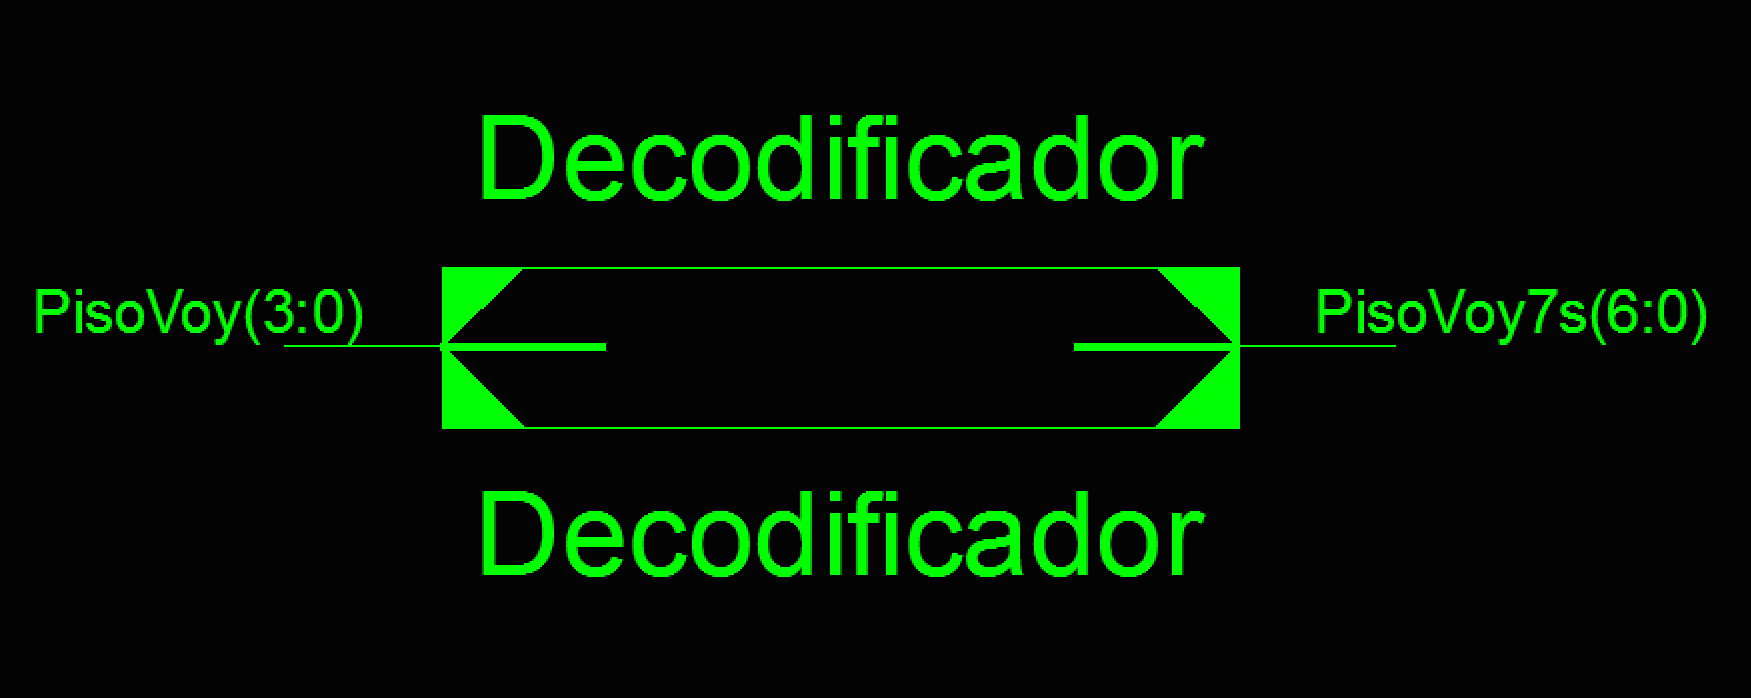
\includegraphics[width = 0.6\textwidth ]{BloqueDecodificador7sOK}
		    \caption{Esquema exterior del bloque Decodificador7s}
		    \label{fig:BloqueDecodificador7sOK}
	\end{figure}
    Además podemos ver en la Figura (\ref{fig:BloqueDecodificador7sImplementacion}) como se compone internamente el bloque, como se codifica en hardware esta utilidad:
    \begin{figure}[H]
		    \centering
		    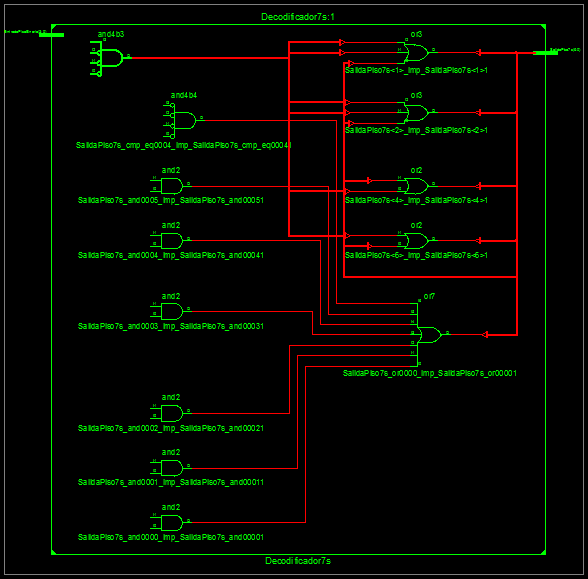
\includegraphics[width = 0.9\textwidth ]{BloqueDecodificador7sImplementacion}
		    \caption{Esquema interno del bloque Decodificador7s}
		    \label{fig:BloqueDecodificador7sImplementacion}
	\end{figure}

\subsection{Código Bloque \textit{Decodificador a 7 segmentos (testbench)}:} \label{code:Decodificador7s_tb}
	
	\inputminted[frame=lines,fontsize=\footnotesize,linenos]{vhdl}{CodeFiles/Decodificador7s_tb.vhd}
	
	Utilizando este testbench se obtiene el comportamiento que se puede ver en la Figura (\ref{fig:SimulacionDecodificador7s}):

    \begin{figure}[H]
		    \centering
		    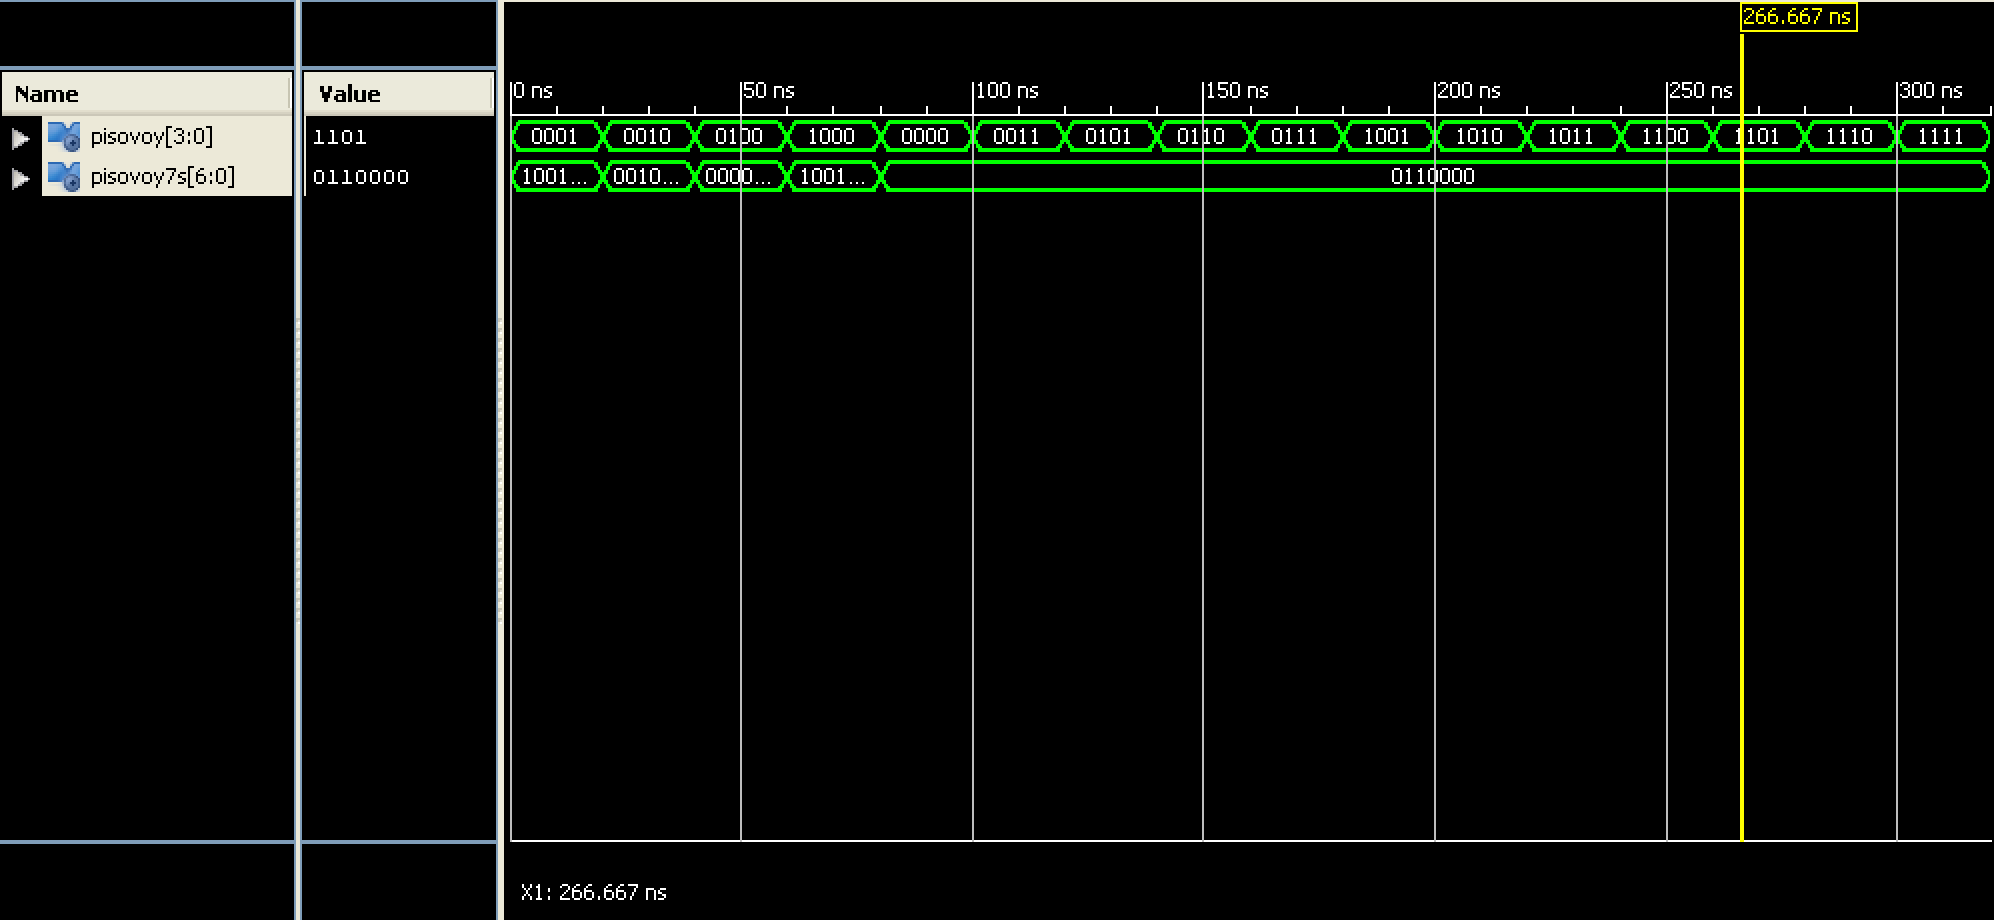
\includegraphics[width = 0.8\textwidth ]{SimulacionDecodificador7s}
		    \caption{Simulación del testbench del bloque Decodificador7s}
		    \label{fig:SimulacionDecodificador7s}
	\end{figure}

	Para entender el comportamiento obtenido en la simulación debemos recordar, el Cuadro (\ref{tab:tabla1ApendiceA}) del Apéndice \ref{app:codEntSal} y el Cuadro (\ref{tab:tabla1ApendiceB}) del Apéndice \ref{app:7segmentos} donde podemos ver como se codifican internamente el número de piso en 4 bits y el número de piso en binario para mostrar la información en el Display 7 segmentos. \\
	
	Según podemos observar logramos la conducta deseada: piso 1 la salida es el carácter 1, piso 2 la salida carácter 2, piso 3 la salida carácter 3, piso 4 la salida carácter 4 y comprobamos que al introducir entradas erróneas la salida es el carácter error.

\subsection{Código Bloque \textit{Alternador de displays}:} \label{code:AlternadorDisplay}
	Como se ha visto en la seccción (\ref{subsection:Spartan-3}) los cuatro displays comparten la salida de 7 bits, cambiando de un display a otro a través de los ánodos de contro. En este bloque se va alternando de un ánodo a otro para mostrar por cada display la salida correspondiente sin que se pise la información y a una frecuencia suficiente para que el parpadeo no sea apreciable. A continuación se puede ver el código que codifica esta funcionalidad: \\ 

	\inputminted[frame=lines,fontsize=\footnotesize,linenos]{vhdl}{CodeFiles/AlternadorDisplay.vhd}
	
		Como se puede ver en la Figura (\ref{fig:BloqueAlternadorDisplayOK}) el esquema obtenido una vez programado y sintetizado se corresponde con el que se pretendía.
    \begin{figure}[H]
		    \centering
		    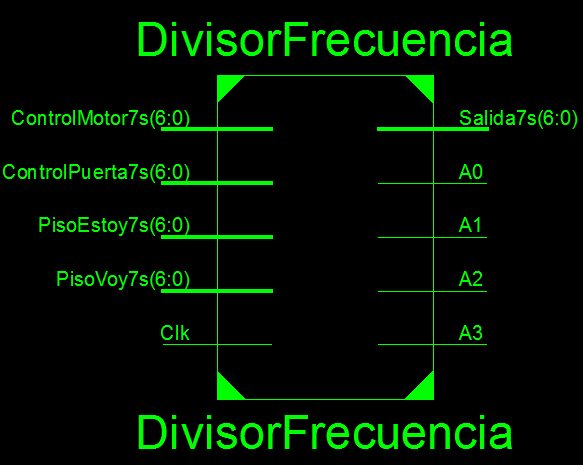
\includegraphics[width = 0.6\textwidth ]{BloqueAlternadorDisplayOK}
		    \caption{Esquema exterior del bloque AlternadorDisplay}
		    \label{fig:BloqueAlternadorDisplayOK}
	\end{figure}
    Además podemos ver en la Figura (\ref{fig:BloqueAlternadorDisplayImplementacion}) como se compone internamente el bloque, como se codifica en hardware esta utilidad:
    \begin{figure}[H]
		    \centering
		    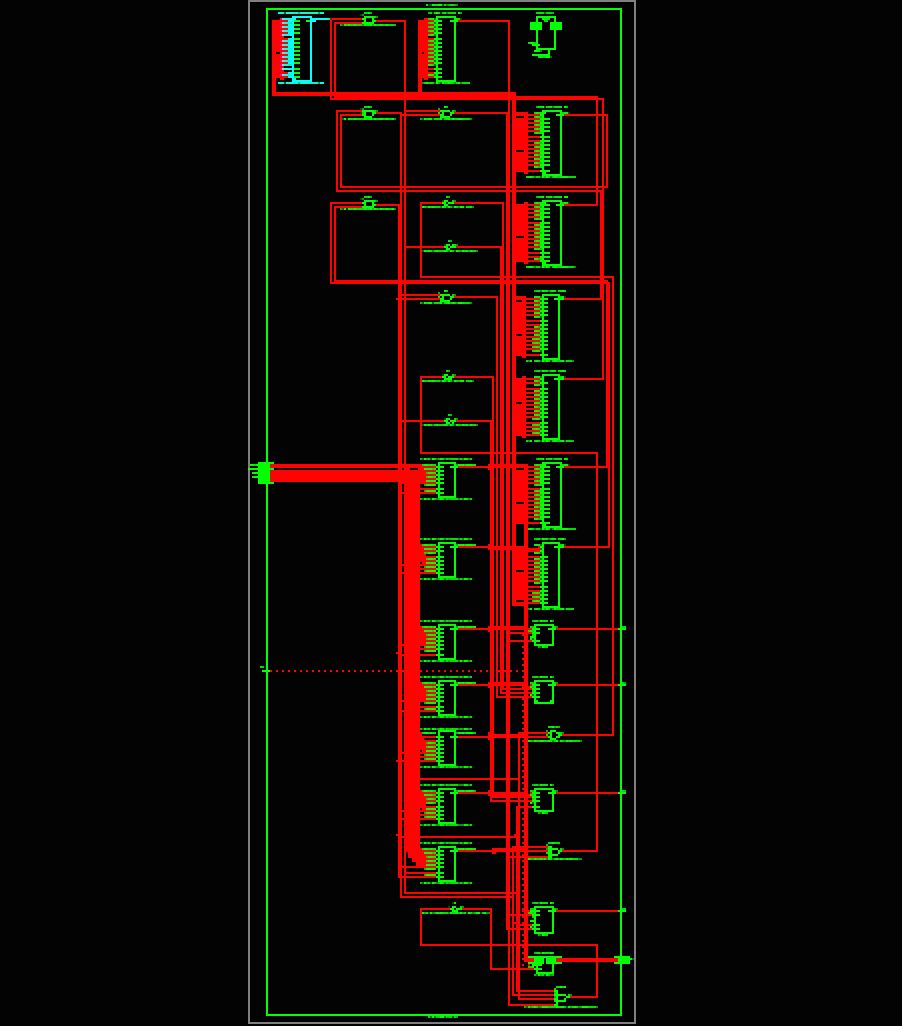
\includegraphics[width = 0.9\textwidth ]{BloqueAlternadorDisplayImplementacion}
		    \caption{Esquema interno del bloque AlternadorDisplay}
		    \label{fig:BloqueAlternadorDisplayImplementacion}
	\end{figure}

\subsection{Código Bloque \textit{Alternador de displays (testbench)}:} \label{code:AlternadorDisplay_Tb}
	\inputminted[frame=lines,fontsize=\footnotesize,linenos]{vhdl}{CodeFiles/AlternadorDisplay_tb.vhd}
	
		Utilizando este testbench se obtiene el comportamiento que se puede ver en la Figura (\ref{fig:SimulacionAlternadorDisplay}):

    \begin{figure}[H]
		    \centering
		    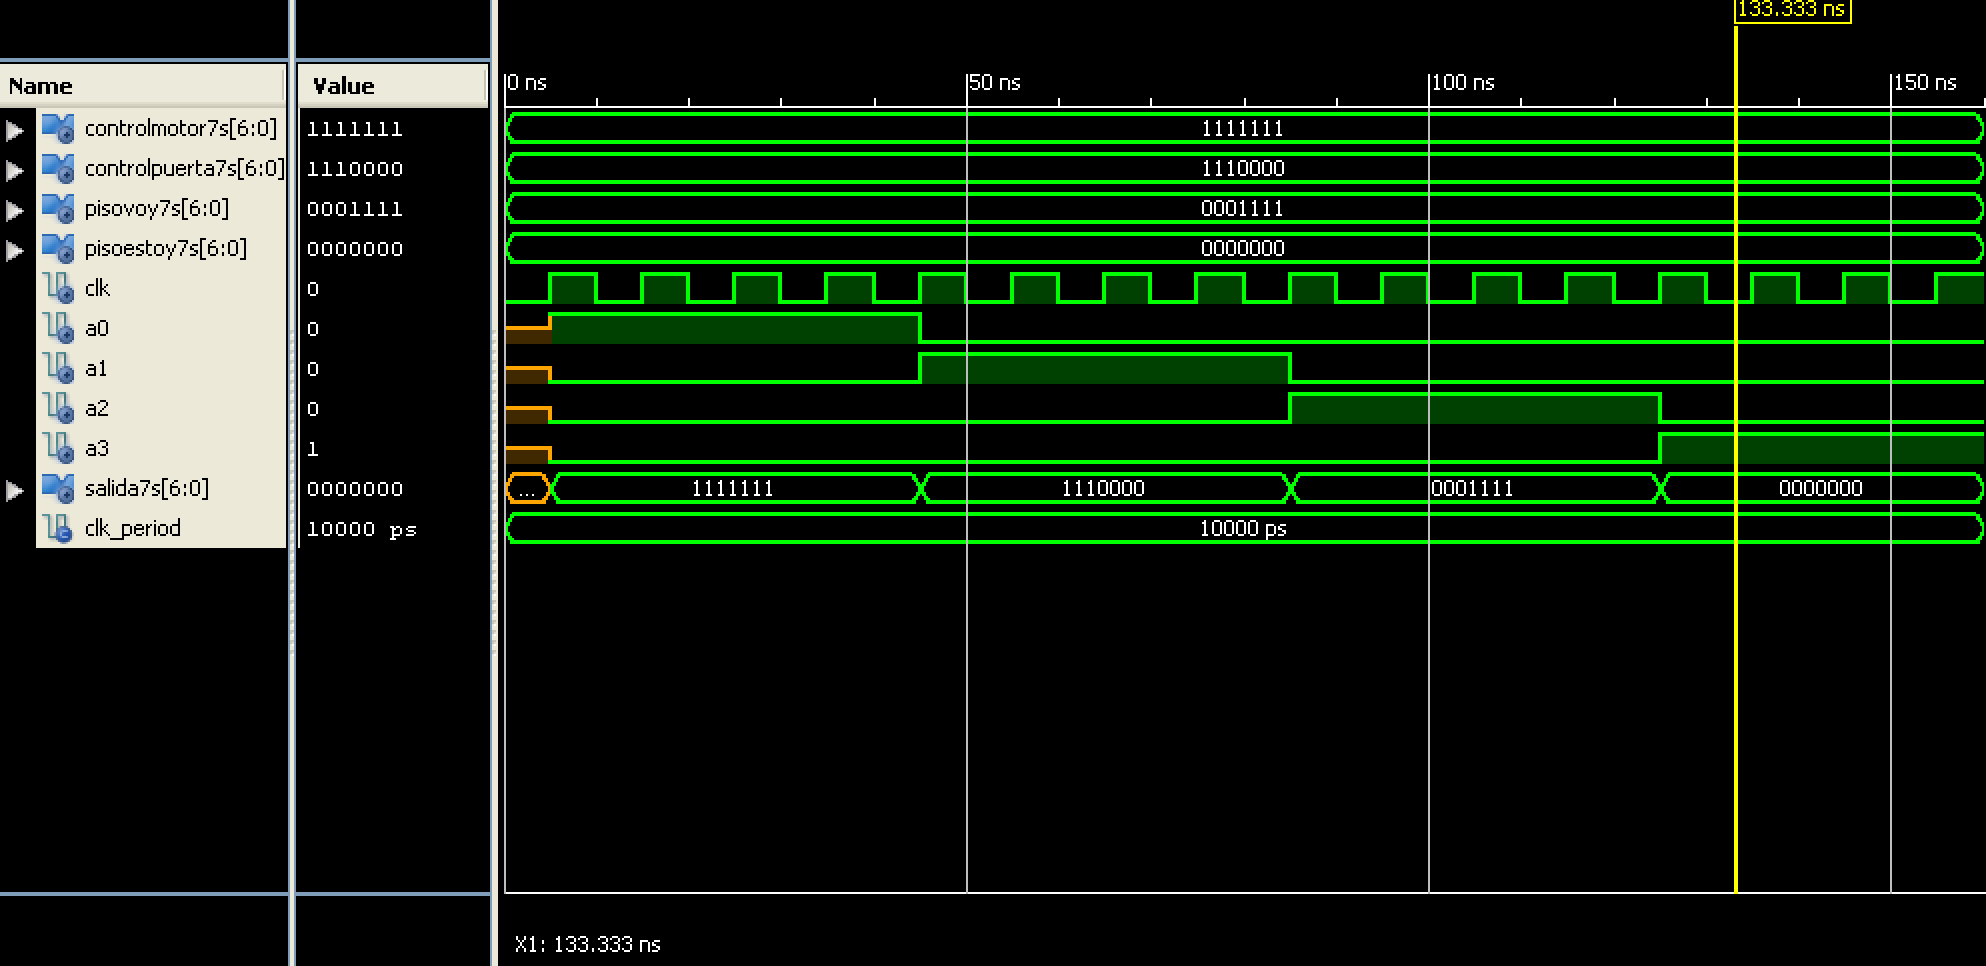
\includegraphics[width = 0.8\textwidth ]{SimulacionAlternadorDisplay}
		    \caption{Simulación del testbench del bloque AlternadorDisplay}
		    \label{fig:SimulacionAlternadorDisplay}
	\end{figure}

\subsection{Código Bloque \textit{PistoActual}:} \label{code:PisoActual}
	Como se ha explicado en la sección (\ref{bloque:PisoActual}) este bloque filtrará posibles lecturas que no nos interese pasar al comparador. De esta forma solo tomará como válidas los vectores que se correspondan con ela codificación de cada piso. Cuando entre una lectura que no se corresponde con ello se pasará el último piso detectado. Esta situación incluye cuando el ascensor de encuentra entre dos pisos (SensorEstoy = 0000) o posibles errores incoherentes que puedan darse debido a la electrónica como podría ser una lectura con valores "0110" o similar. A continuación se puede ver el código que codifica dichas funcionalidades: \\ 

    \inputminted[frame=lines,fontsize=\footnotesize,linenos]{vhdl}{CodeFiles/PisoActual.vhd}
    
    Como se puede ver en la Figura (\ref{fig:BloquePisoActualOK}) el esquema obtenido una vez programado y sintetizado se corresponde con el que se pretendía.
    \begin{figure}[H]
		    \centering
		    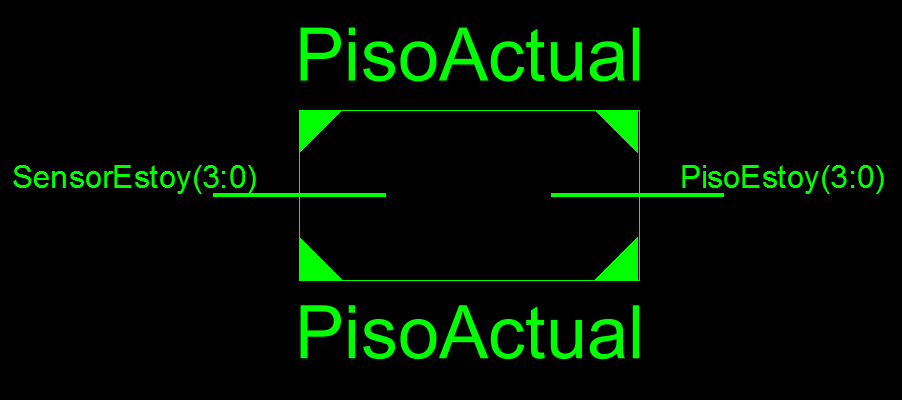
\includegraphics[width = 0.6\textwidth ]{BloquePisoActualOK}
		    \caption{Esquema exterior del bloque Piso Actual}
		    \label{fig:BloquePisoActualOK}
	\end{figure}
    Además podemos ver en la Figura (\ref{fig:BloquePisoActualImplementacion}) como se compone internamente el bloque, como se codifica en hardware esta utilidad:
    \begin{figure}[H]
		    \centering
		    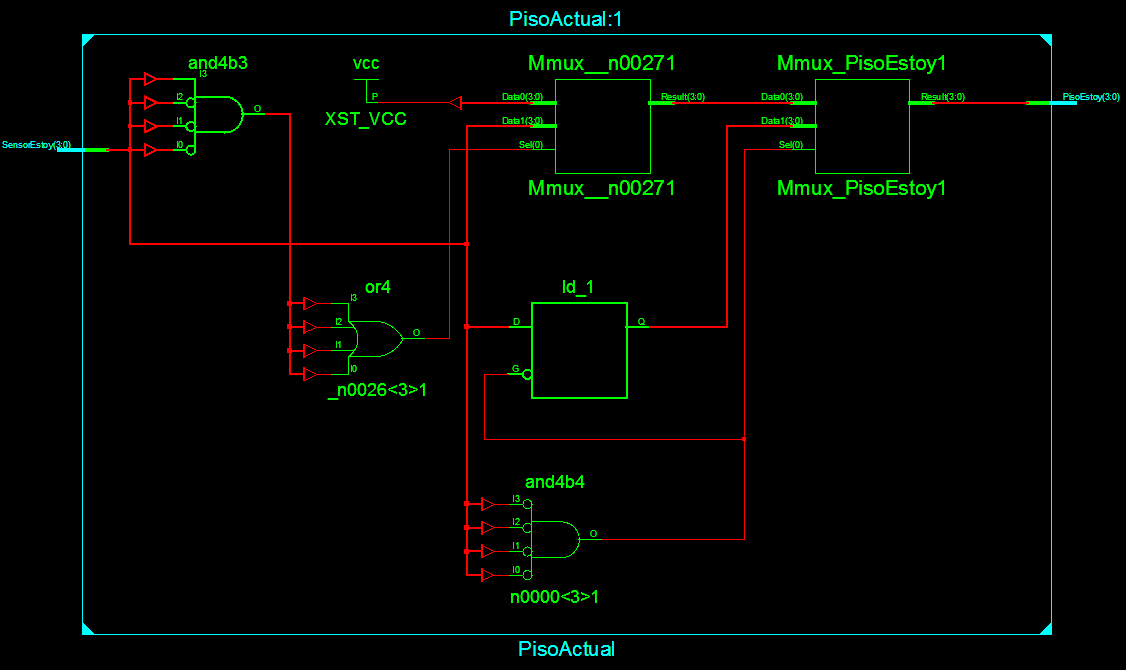
\includegraphics[width = 0.9\textwidth ]{BloquePisoActualImplementacion}
		    \caption{Esquema interno del bloque Piso Actual}
		    \label{fig:BloquePisoActualImplementacion}
	\end{figure}

\subsection{Código Bloque \textit{PistoActual (testbench)}:} \label{code:PisoActual_tb}
    \inputminted[frame=lines,fontsize=\footnotesize,linenos]{vhdl}{CodeFiles/PisoActual_tb.vhd}
    
    Utilizando este testbench se obtiene el comportamiento que se puede ver en la Figura (\ref{fig:SimulacionPisoActual}):

    \begin{figure}[H]
		    \centering
		    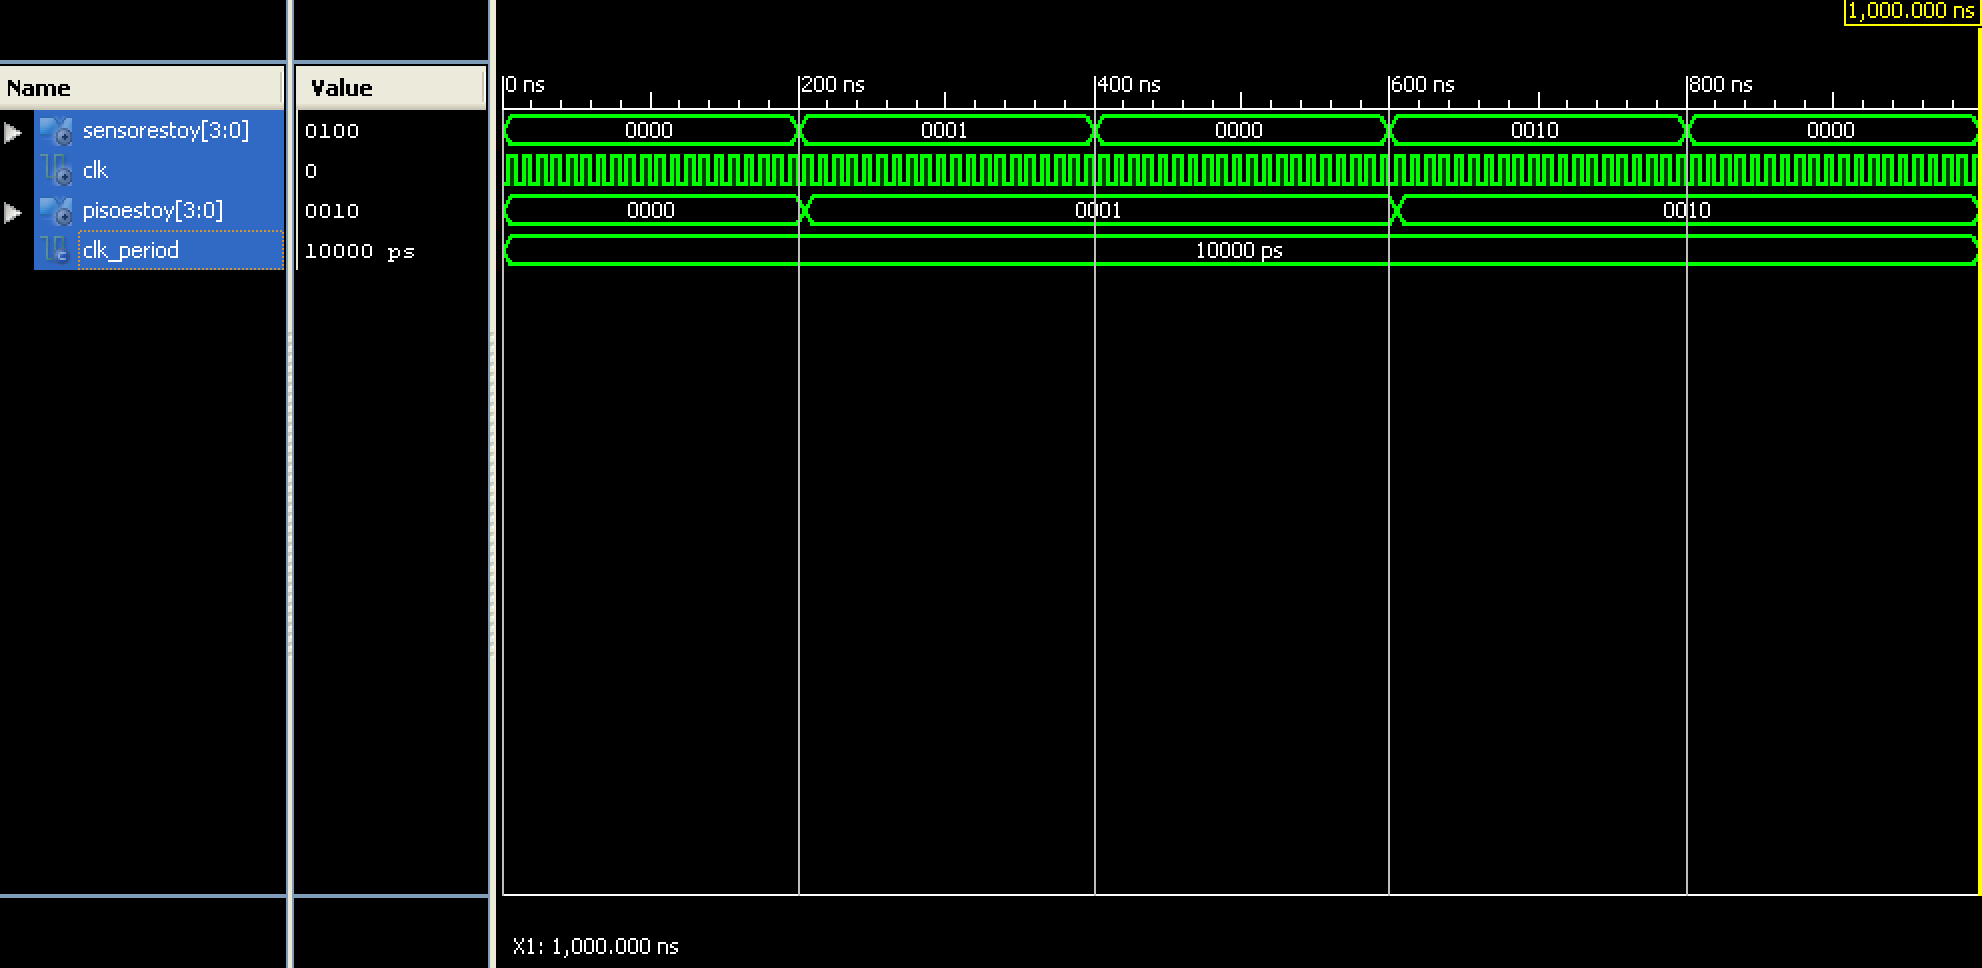
\includegraphics[width = 0.8\textwidth ]{SimulacionPisoActual}
		    \caption{Simulación del testbench del bloque PisoActual}
		    \label{fig:SimulacionPisoActual}
	\end{figure}


\subsection{Código Bloque \textit{Bloqueador PisoVoy}:} \label{code:BloqueadorpisoVoy}

    Como se ha adelantado en la sección (\ref{bloque:BloqueadorPisoVoy}) este bloque es el encargado de filtrar posibles lecturas que no nos interesen pasar al comparador y almacenar hasta tres lecturas válidas. Al poderse almacenar más de una lectura solo se tomarán como lecturas válidas los vectores que se correspondan con la codificación de cada piso, no son válidas dos pisos seguidos iguales. \\
    
    Cuando entre una lectura que no se corresponda con un piso se pasará el último piso válido detectado,  esta situación incluye tanto no llamarle desde ningún piso como posibles errores incoherentes que puedan darse, por ejemplo llamarlo simultáneamente desde más de un piso. \\
    
	En el momento que el ascensor está parado comprueba si hay valores almacenados, en dicho caso espera un tiempo y carga uno de ellos (en un orden determinado) en la salida que va al comparador. Sin embargo si no los hay la salida se mantiene en la última posición hasta que se introduce un nuevo piso. No obstante si está en movimiento la salida que va al comparador se mantiene constante, mientras que puedes almacenar un par de pisos más en dos variables diferentes.
	
    \inputminted[frame=lines,fontsize=\footnotesize,linenos]{vhdl}{CodeFiles/BloqueadorPisoVoy.vhd}
	Como se puede ver en la Figura (\ref{fig:BloqueBloqueadorPisoVoyOK}) el esquema obtenido una vez programado y sintetizado se corresponde con el que se pretendía.
    \begin{figure}[H]
		    \centering
		    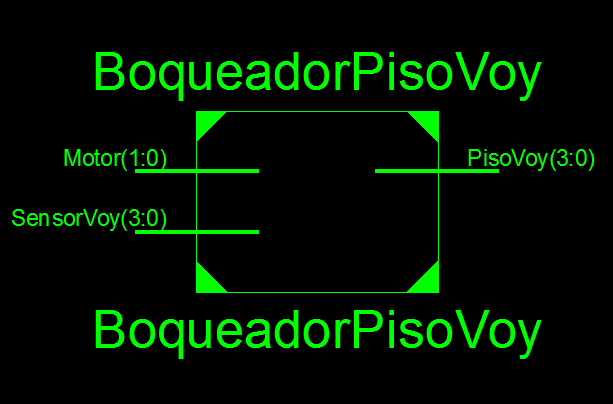
\includegraphics[width = 0.6\textwidth ]{BloqueBloqueadorPisoVoyOK}
		    \caption{Esquema exterior del bloque Bloqueador PisoVoy}
		    \label{fig:BloqueBloqueadorPisoVoyOK}
	\end{figure}
    Además podemos ver en la Figura (\ref{fig:BloqueBloqueadorPisoVoyImplementacion}) como se compone internamente el bloque, como se codifica en hardware esta utilidad:
    \begin{figure}[H]
		    \centering
		    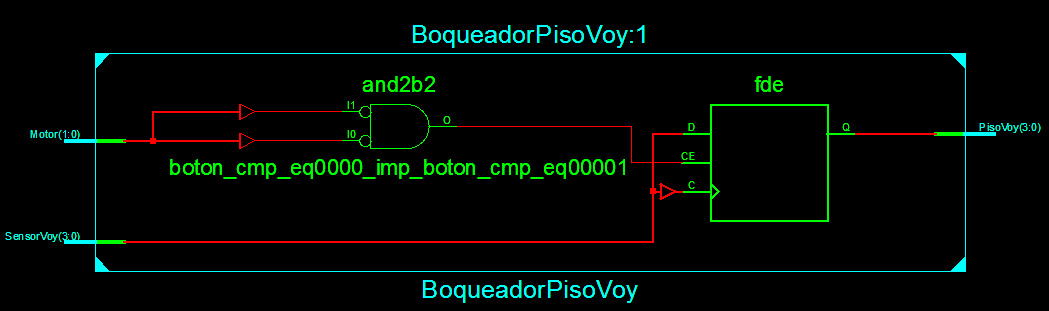
\includegraphics[width = 0.9\textwidth ]{BloqueBloqueadorPisoVoyImplementacion}
		    \caption{Esquema interno del bloque Bloqueador PisoVoy}
		    \label{fig:BloqueBloqueadorPisoVoyImplementacion}
	\end{figure}

\subsection{Código Bloque \textit{Bloqueador PisoVoy (testbench)}:} \label{code:BloqueadorpisoVoy_tb}
    \inputminted[frame=lines,fontsize=\footnotesize,linenos]{vhdl}{CodeFiles/BloqueadorPisoVoy_tb.vhd}

    Utilizando este testbench se obtiene el comportamiento que se puede ver en la Figura (\ref{fig:SimulacionBloqueadorPisoVoy}):

    \begin{figure}[H]
		    \centering
		    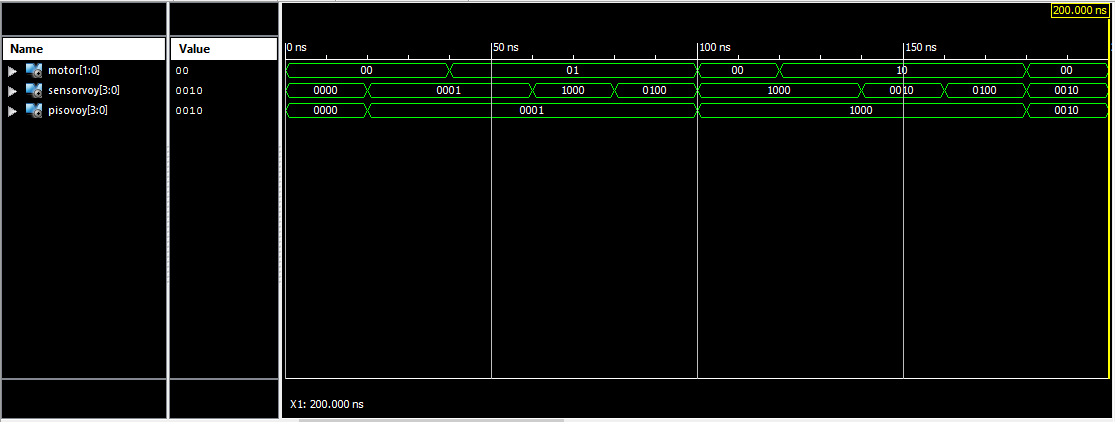
\includegraphics[width = 0.8\textwidth ]{SimulacionBloqueadorPisoVoy}
		    \caption{Simulación del testbench del bloque BloqueadorPisoVoy}
		    \label{fig:SimulacionBloqueadorPisoVoy}
	\end{figure}

    Para entender el comportamiento obtenido en la simulación debemos recordar, el Cuadro (\ref{tab:tabla1ApendiceA}) del Apéndice \ref{app:codEntSal} y el Cuadro (\ref{tab:tabla2ApendiceA}) del Apéndice \ref{app:codEntSal} donde podemos ver como se codifican internamente el número de piso y el funcionamiento del motor. 
	Según podemos observar obtenemos el comportamiento deseado:
	\begin{itemize}
	    \item Ascensor Parado y nada pulsado se mantiene la situación donde se inicializa.
	    \item Ascensor Parado y pulso planta 2 se guarda en PisoVoy la planta pulsada.
	    \item Ascensor en movimiento y nada pulsado se mantiene la situación anterior.
	    \item Ascensor en movimiento y pulso planta 4: PisoVoy "lleno" se guarda en MemPisoVoy1 la planta pulsada.
	    \item Ascensor en movimiento y pulso planta 1: PisoVoy y MemPisoVoy1 "lleno" se guarda en MemPisoVoy2 la planta pulsada.
	    \item Ascensor en movimiento y nada pulsado.
	    \item Ascensor Parado y nada pulsado mantiene un tiempo la situación anterior.
	    \item Ascensor Parado, nada pulsado: MemPisoVoy1 "lleno", tras pasar el tiempo delay pasa el dato de MemPisoVoy1 a PisoVoy (en un ciclo de reloj). 
	    \item Ascensor Parado, nada pulsado: MemPisoVoy2 "lleno" pasa el dato de MemPisoVoy2 a MemPisoVoy1 (en un ciclo de reloj).
	    \item Ascensor en movimiento y nada pulsado.				 
	    \item Ascensor Parado y nada pulsado mantiene un tiempo la situación anterior.
	    \item Ascensor Parado, nada pulsado: MemPisoVoy1 "lleno", tras pasar el tiempo delay pasa el dato de MemPisoVoy1 a PisoVoy (en un ciclo de reloj). 
	    \item Ascensor Parado, nada pulsado: MemPisoVoy2 "vacío" pasa el dato de MemPisoVoy2 a MemPisoVoy1 (en un ciclo de reloj).
	    \item Ascensor en movimiento y nada pulsado.
	    \item Ascensor Parado y nada pulsado y nada en variables de almacenamiento se mantiene la situación anterior.
	\end{itemize}

\subsection{Código Bloque \textit{Decodificador Binario a Entero}:} \label{code:DecodificadorBinarioEntero}
	Como se ha visto en la sección (\ref{bloque:DecodificadorBinarioEntero}) este bloque pasa de la codificación binaria que se ha dado a cada piso a su equivalente entero para su posterior comparación. Se puede ver el código de dicho bloque a continuación: \\ 

    \inputminted[frame=lines,fontsize=\footnotesize,linenos]{vhdl}{CodeFiles/DecodificadorBinarioEntero.vhd}
    
    Como se puede ver en la Figura (\ref{fig:BloqueDecodificadorBinarioEnteroOK}) el esquema obtenido una vez programado y sintetizado se corresponde con el que se pretendía.
    \begin{figure}[H]
		    \centering
		    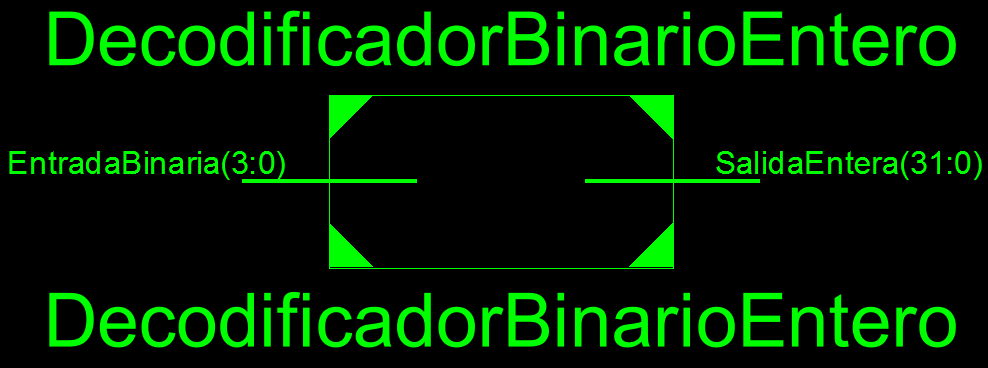
\includegraphics[width = 0.6\textwidth ]{BloqueDecodificadorBinarioEnteroOK}
		    \caption{Esquema exterior del bloque Decodificador Binario-Entero}
		    \label{fig:BloqueDecodificadorBinarioEnteroOK}
	\end{figure}
    Además podemos ver en la Figura (\ref{fig:BloqueDecodificadorBinarioEnteroImplementacion}) como se compone internamente el bloque, como se codifica en hardware esta utilidad:
    \begin{figure}[H]
		    \centering
		    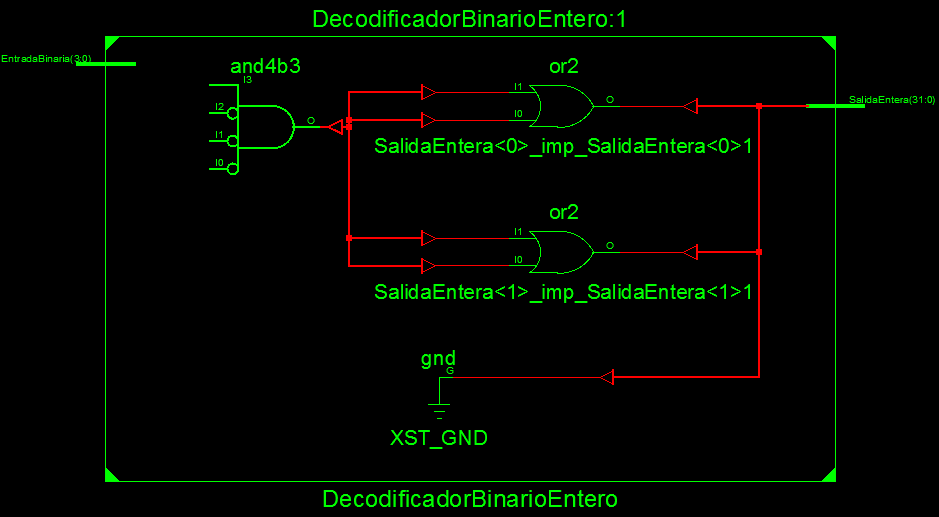
\includegraphics[width = 0.9\textwidth ]{BloqueDecodificadorBinarioEnteroImplementacion}
		    \caption{Esquema interno del bloque Decodificador Binario-Entero}
		    \label{fig:BloqueDecodificadorBinarioEnteroImplementacion}
	\end{figure}
    
\subsection{Código Bloque \textit{Decodificador Binario a Entero (testbench)}:} \label{code:DecodificadorBinarioEntero_tb}
    \inputminted[frame=lines,fontsize=\footnotesize,linenos]{vhdl}{CodeFiles/DecodificadorBinarioEntero_tb.vhd}

    Utilizando este testbench se obtiene el comportamiento que se puede ver en la Figura (\ref{fig:SimulacionDecodificadorBinarioEntero}):

    \begin{figure}[H]
		    \centering
		    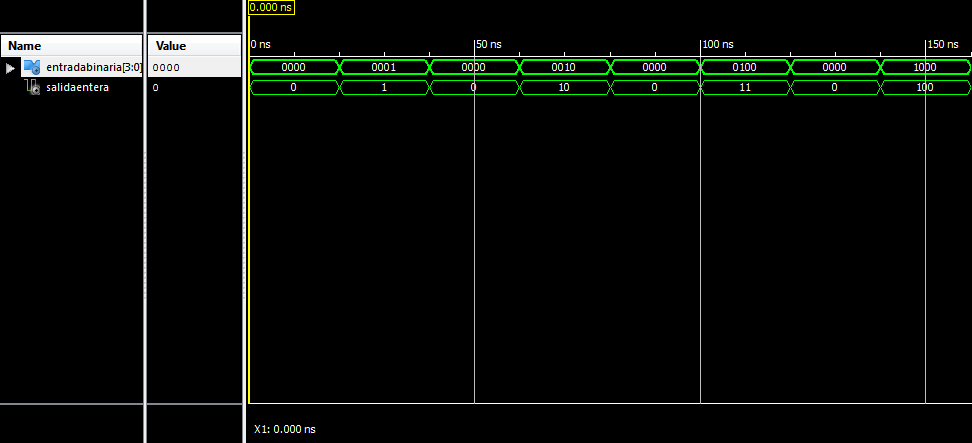
\includegraphics[width = 0.8\textwidth ]{SimulacionDecodificadorBinarioEntero}
		    \caption{Simulación del testbench del bloque DecodificadorBinarioEntero}
		    \label{fig:SimulacionDecodificadorBinarioEntero}
	\end{figure}

\subsection{Código Bloque \textit{Comparador}:} \label{code:Comparador}
	Como se ha visto en la seccion (\ref{bloque:Comparado}) este bloque compara las dos señales enteras; si el piso objetivo está por encima del actual el motor sube y la puerta se cierra, si el piso objetivo es igual al piso actual el motor está parado y la puerta abierta, y finalmente, si el piso objetivo es menor que el piso actual el motor baja manteniendo la puerta cerrada durante el proceso. A continuación se presenta el código del bloque: \\ 

    \inputminted[frame=lines,fontsize=\footnotesize,linenos]{vhdl}{CodeFiles/Comparador.vhd}	

	Como se puede ver en la Figura (\ref{fig:BloqueComparadorOK}) el esquema obtenido una vez programado y sintetizado se corresponde con el que se pretendía.
    \begin{figure}[H]
		    \centering
		    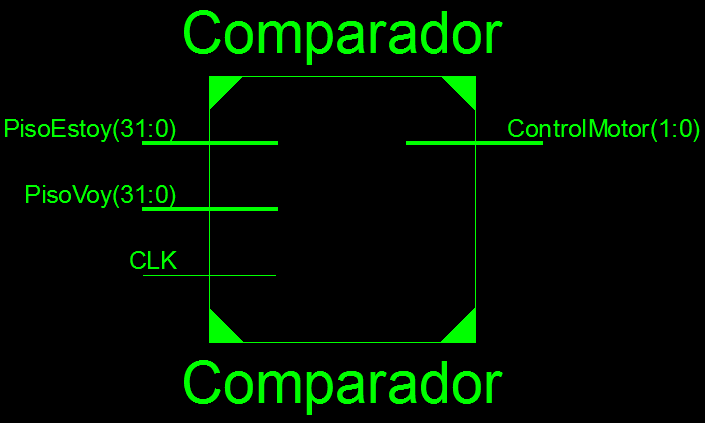
\includegraphics[width = 0.6\textwidth ]{BloqueComparadorOK}
		    \caption{Esquema exterior del Bloque Comparador}
		    \label{fig:BloqueComparadorOK}
	\end{figure}
    Además podemos ver en la Figura (\ref{fig:BloqueComparadorImplementacion}) como se compone internamente el bloque, como se codifica en hardware esta utilidad:
    \begin{figure}[H]
		    \centering
		    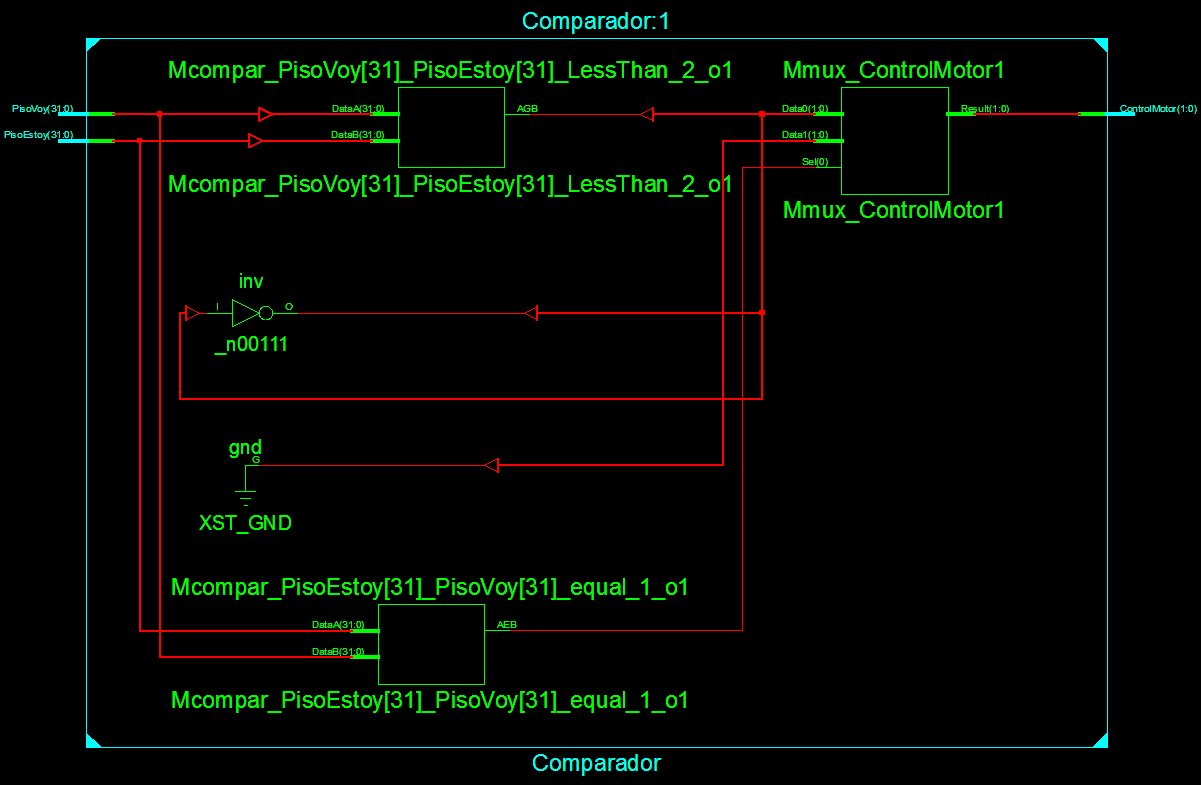
\includegraphics[width = 0.9\textwidth ]{BloqueComparadorImplementacion}
		    \caption{Esquema interno del Bloque Comparador}
		    \label{fig:BloqueComparadorImplementacion}
	\end{figure}

\subsection{Código Bloque \textit{Comparador (testbench)}:} \label{code:Comparador_tb}
    \inputminted[frame=lines,fontsize=\footnotesize,linenos]{vhdl}{CodeFiles/Comparador_tb.vhd}

    Utilizando este testbench se obtiene el comportamiento que se puede ver en la Figura (\ref{fig:SimulacionComparador}):

    \begin{figure}[H]
		    \centering
		    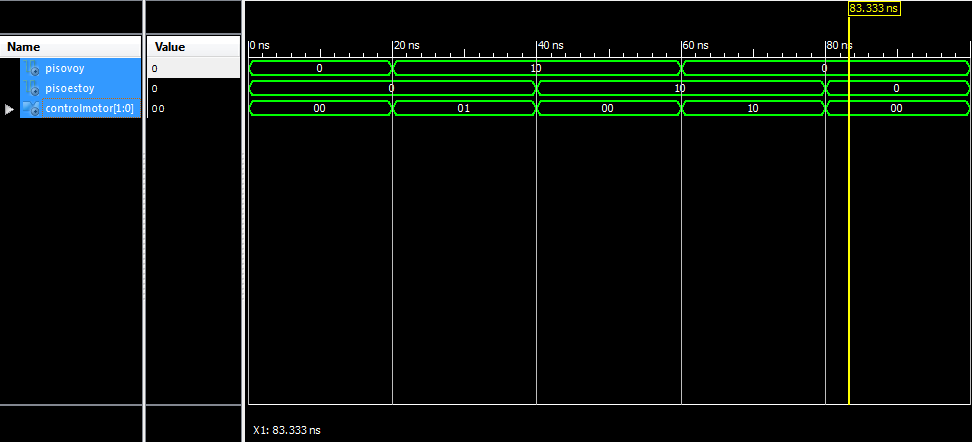
\includegraphics[width = 0.8\textwidth ]{SimulacionComparador}
		    \caption{Simulación del testbench del bloque Comparador}
		    \label{fig:SimulacionComparador}
	\end{figure}

\subsection{Código Bloque \textit{ Simulacion Motor Puerta}:} \label{code:MotorPuerta}
	Como se ha visto en la sección (\ref{boque:MotorPuerta}) al no tener motor y puerta reales se ha optado por sacar su reacción a traves de los displays. Este bloque es similar al bloque Decodificador7s (se puede encontrar la descripción en la seccion \ref{bloque:Decodificador7s} así como su codificación en la sección \ref{code:Decodificador7s} para observar las similitudes). Lo que hace es tomar la señal de entrada de dos bits, que codifica la reacción del motor y la puerta para transformarla en un caracter que se podrá mostrar a través del display de 7 segmentos. La codificación en VHDL se puede ver a continuación: \\ 

	\inputminted[frame=lines,fontsize=\footnotesize,linenos]{vhdl}{CodeFiles/MotorPuerta.vhd}

	Como se puede ver en la Figura (\ref{fig:MotorPuertaOK}) el esquema obtenido una vez programado y sintetizado se corresponde con el que se pretendía.
    \begin{figure}[H]
		    \centering
		    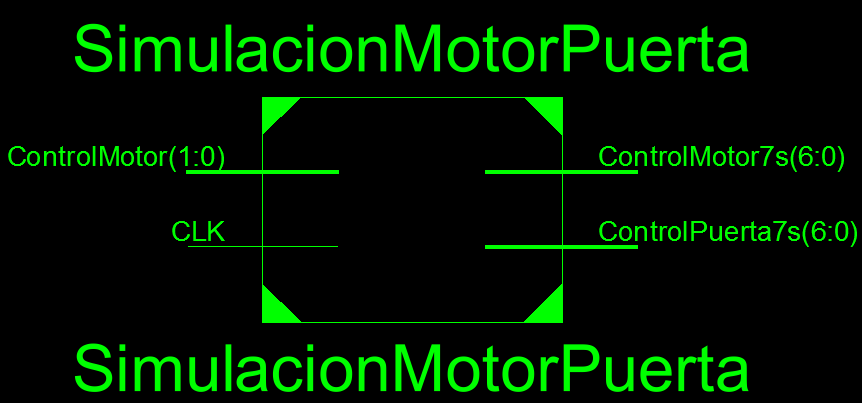
\includegraphics[width = 0.6\textwidth ]{MotorPuertaOK}
		    \caption{Esquema exterior del simulador Motor Puerta}
		    \label{fig:MotorPuertaOK}
	\end{figure}
    Además podemos ver en la Figura (\ref{fig:MotorPuertaImplementacion}) como se compone internamente el bloque, como se codifica en hardware esta utilidad:
    \begin{figure}[H]
		    \centering
		    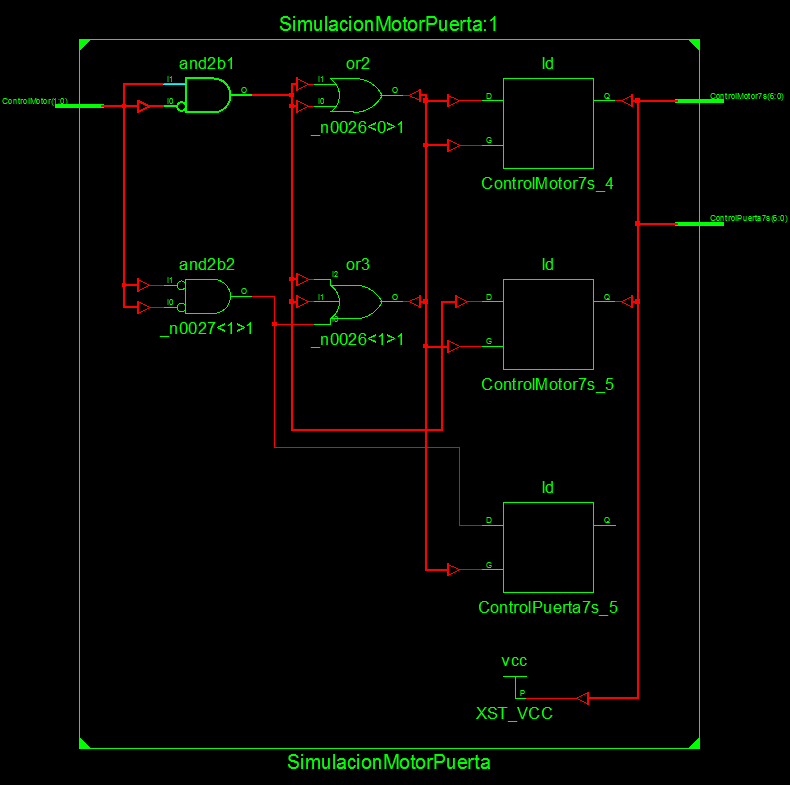
\includegraphics[width = 0.9\textwidth ]{MotorPuertaImplementacion}
		    \caption{Esquema interno del simulador Motor Puerta}
		    \label{fig:MotorPuertaImplementacion}
	\end{figure}
\subsection{Código Bloque \textit{Simulacion Motor Puerta (testbench)}:} \label{code:MotorPuerta_tb}
	\inputminted[frame=lines,fontsize=\footnotesize,linenos]{vhdl}{CodeFiles/MotorPuerta_tb.vhd}

    Utilizando este testbench se obtiene el comportamiento que se puede ver en la Figura (\ref{fig:SimulacionMotorPuerta}):

    \begin{figure}[H]
		    \centering
		    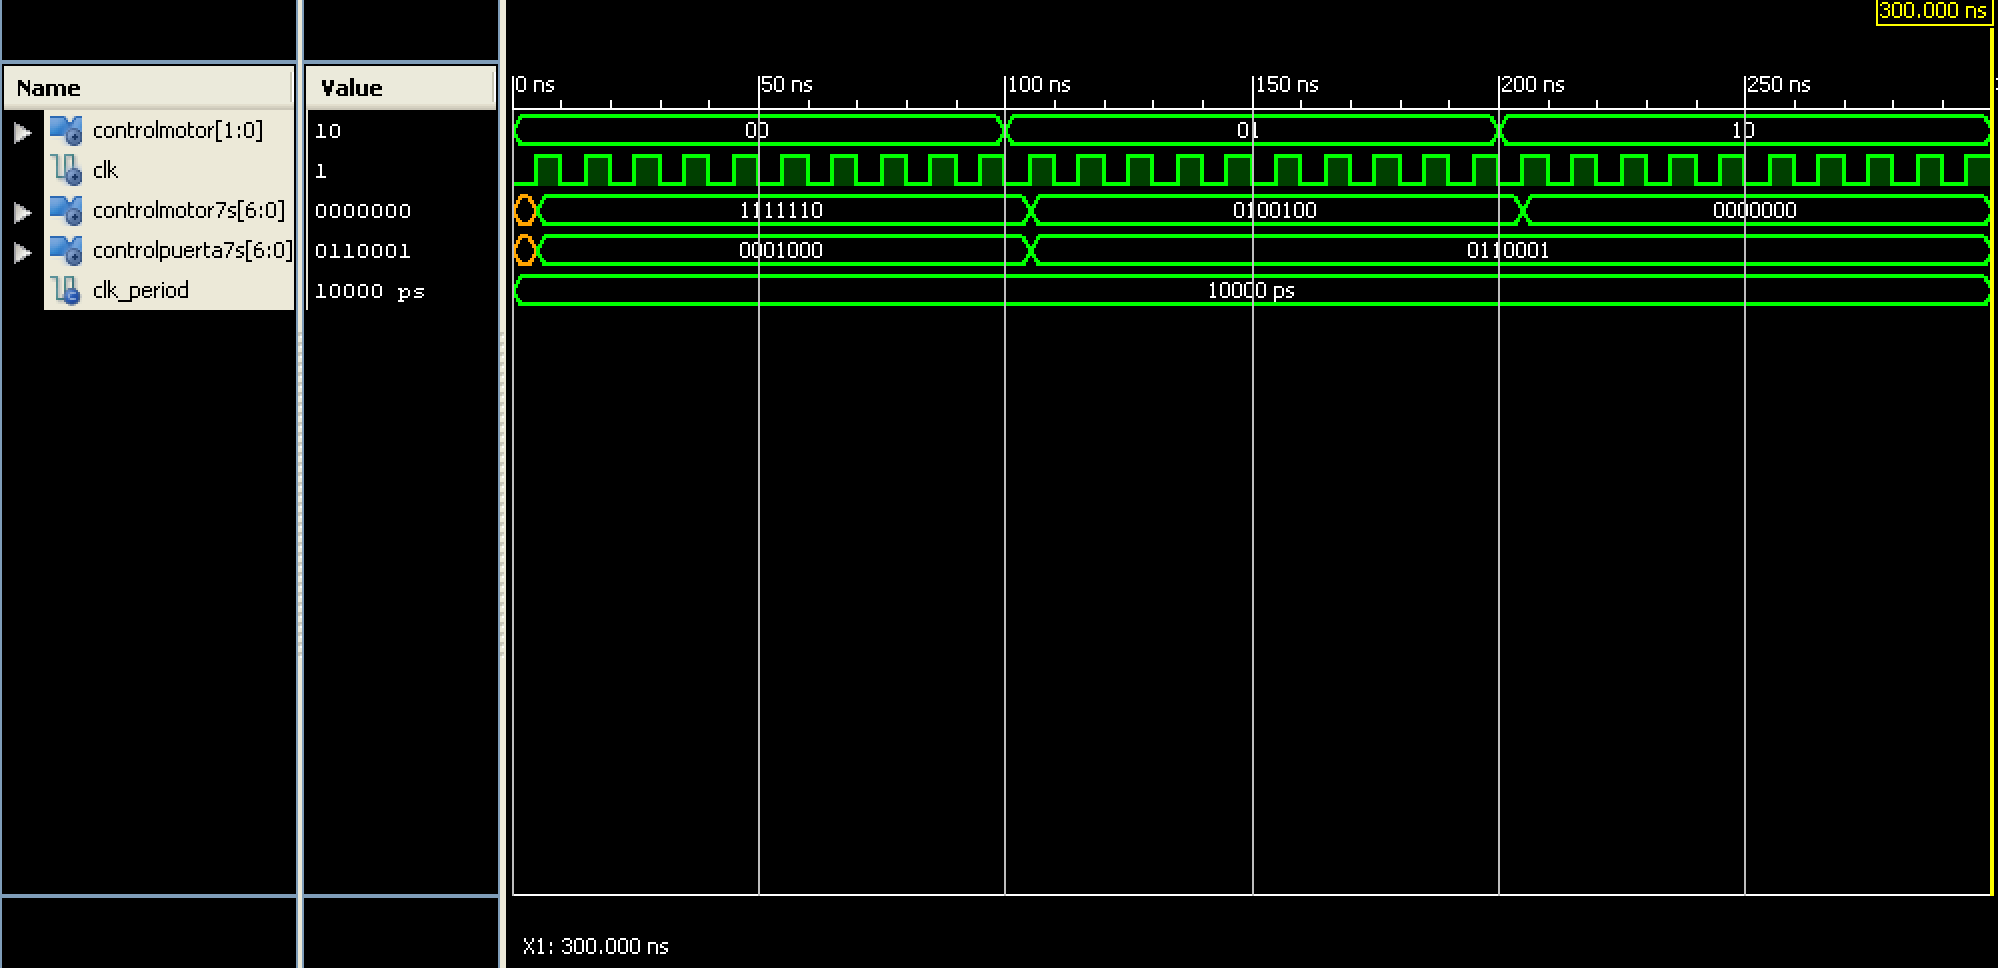
\includegraphics[width = 0.8\textwidth ]{SimulacionPuertaMotor}
		    \caption{Simulación del testbench del simulador MotorPuerta}
		    \label{fig:SimulacionMotorPuerta}
	\end{figure}

\subsection{Entidad \textit{Interfaz Entrada}:} \label{code:InterfazEntrada}
	\inputminted[frame=lines,fontsize=\footnotesize,linenos]{vhdl}{CodeFiles/EntidadInterfazEntrada.vhd}

	Como se puede ver en la Figura (\ref{fig:EntidadInterfazEntradaOK}) el esquema obtenido una vez programado y sintetizado se corresponde con el que se pretendía.
    \begin{figure}[H]
		    \centering
		    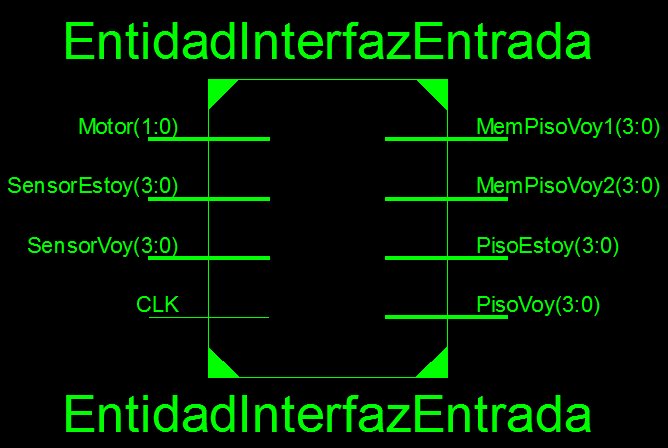
\includegraphics[width = 0.6\textwidth ]{EntidadInterfazEntradaOK}
		    \caption{Esquema exterior de la Entidad InterfazEntrada}
		    \label{fig:EntidadInterfazEntradaOK}
	\end{figure}
    Además podemos ver en la Figura (\ref{fig:EntidadInterfazEntradaImplementacion}) como se compone internamente el bloque, como se codifica en hardware esta utilidad:
    \begin{figure}[H]
		    \centering
		    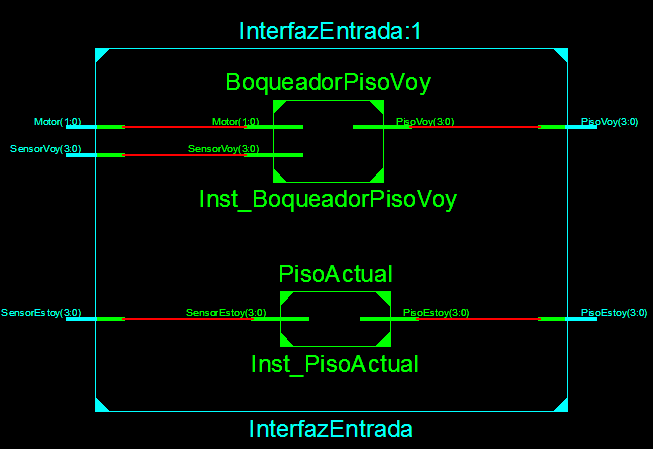
\includegraphics[width = 0.9\textwidth ]{EntidadInterfazEntradaImplementacion}
		    \caption{Esquema interno de la Entidad InterfazEntrada}
		    \label{fig:EntidadInterfazEntradaImplementacion}
	\end{figure}

\subsection{Código Entidad \textit{Interfaz Entrada (testbench)}:} \label{code:InterfazEntrada_tb}
	\inputminted[frame=lines,fontsize=\footnotesize,linenos]{vhdl}{CodeFiles/EntidadInterfazEntrada_tb.vhd}

    Utilizando este testbench se obtiene el comportamiento que se puede ver en la Figura (\ref{fig:SimulacionEntidadInterfazEntrada}):

    \begin{figure}[H]
		    \centering
		    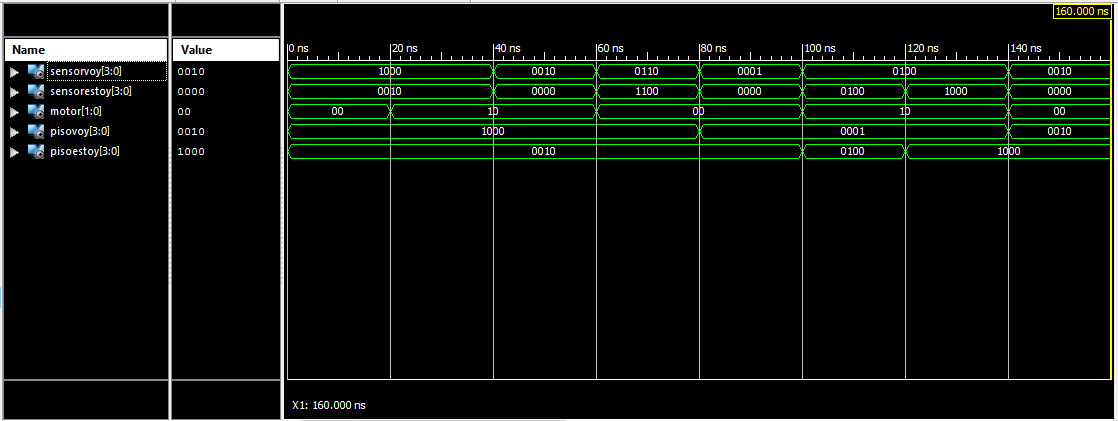
\includegraphics[width = 0.8\textwidth ]{SimulacionEntidadInterfazEntrada}
		    \caption{Simulación del testbench de la entidad InterfazEntrada}
		    \label{fig:SimulacionEntidadInterfazEntrada}
	\end{figure}

\subsection{Código Entidad \textit{Control Ascensor}:} \label{code:ControlAscensor}
	Como se ha explicado en la sección (\ref{bloque:ControlAscensor}) esta entidad coordina y encapsula lo necesario para la toma de decisiones llevada a cabo por nuestro sistema, esto incluye el comparador y el codificador de binario a entero vistos anteriormente. \\ 

	\inputminted[frame=lines,fontsize=\footnotesize,linenos]{vhdl}{CodeFiles/EntidadControlAscensor.vhd}

	Como se puede ver en la Figura (\ref{fig:EntidadControlAscensorOK}) el esquema obtenido una vez programado y sintetizado se corresponde con el que se pretendía.
    \begin{figure}[H]
		    \centering
		    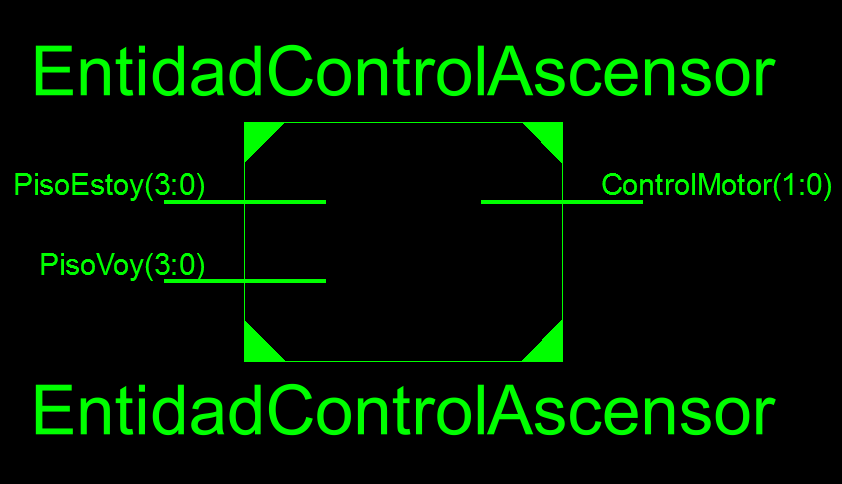
\includegraphics[width = 0.6\textwidth ]{EntidadControlAscensorOK}
		    \caption{Esquema exterior de la Entidad ControlAscensor}
		    \label{fig:EntidadControlAscensorOK}
	\end{figure}
    Además podemos ver en la Figura (\ref{fig:EntidadControlAscensorImplementacion}) como se compone internamente el bloque, como se codifica en hardware esta utilidad:
    \begin{figure}[H]
		    \centering
		    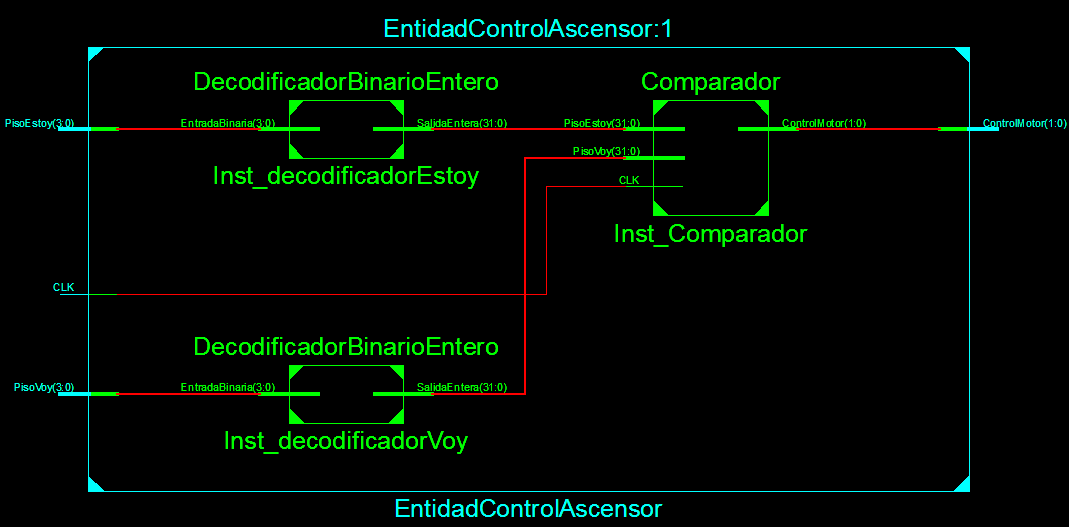
\includegraphics[width = 0.9\textwidth ]{EntidadControlAscensorImplementacion}
		    \caption{Esquema interno de la Entidad ControlAscensor}
		    \label{fig:EntidadControlAscensorImplementacion}
	\end{figure}

\subsection{Código Entidad \textit{Control Ascensor (testbench)}:} \label{code:ControlAscensor_tb}
	\inputminted[frame=lines,fontsize=\footnotesize,linenos]{vhdl}{CodeFiles/EntidadControlAscensor_tb.vhd}

    Utilizando este testbench se obtiene el comportamiento que se puede ver en la Figura (\ref{fig:SimulacionEntidadControlAscensor}):

    \begin{figure}[H]
		    \centering
		    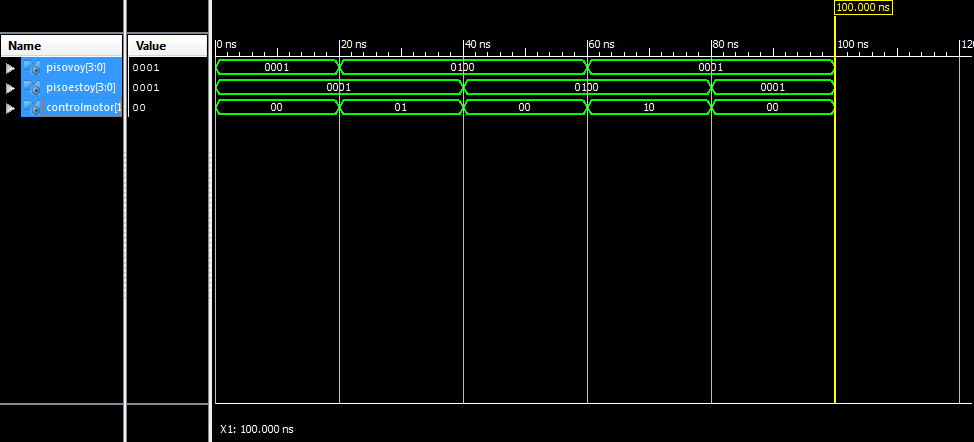
\includegraphics[width = 0.8\textwidth ]{SimulacionEntidadControlAscensor}
		    \caption{Simulación del testbench de la entidad ControlAscensor}
		    \label{fig:SimulacionEntidadControlAscensor}
	\end{figure}

\subsection{Código Entidad \textit{Visualizacion}:} \label{code:Visualizacion}

Esta entidad, formada por tres bloques, dos Decodificador7s y un AlternadorDisplay se encarga de mostrar en las cuatro pantallas de siete segmentos el estado del ascensor. \\ 
	\inputminted[frame=lines,fontsize=\footnotesize,linenos]{vhdl}{CodeFiles/EntidadVisualizacion.vhd}

	Como se puede ver en la Figura (\ref{fig:VisualizacionOK}) el esquema obtenido una vez programado y sintetizado se corresponde con el que se pretendía.
    \begin{figure}[H]
		    \centering
		    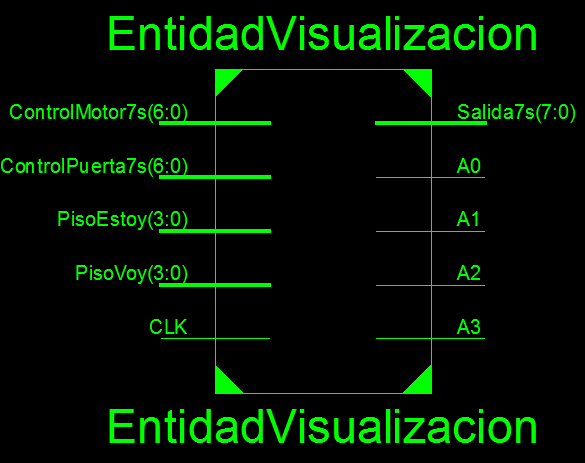
\includegraphics[width = 0.6\textwidth ]{EntidadVisualizacionOK}
		    \caption{Esquema exterior de la Entidad Visualizacion}
		    \label{fig:EntidadVisualizacionOK}
	\end{figure}
    Además podemos ver en la Figura (\ref{fig:EntidadVisualizacionImplementacion}) como se compone internamente el bloque, como se codifica en hardware esta utilidad:
    \begin{figure}[H]
		    \centering
		    \includegraphics[width = 0.9\textwidth ]{EntidadVisualizacion}
		    \caption{Esquema interno de la Entidad Visualizacion}
		    \label{fig:EntidadVisualizacionImplementacion}
	\end{figure}

\subsection{Código Entidad \textit{Visualizacion (testbench)}:} \label{code:Visualizacion_tb}
	\inputminted[frame=lines,fontsize=\footnotesize,linenos]{vhdl}{CodeFiles/EntidadVisualizacion_tb.vhd}

    Utilizando este testbench se obtiene el comportamiento que se puede ver en la Figura (\ref{fig:SimulacionEntidadVisualizacion}):

    \begin{figure}[H]
		    \centering
		    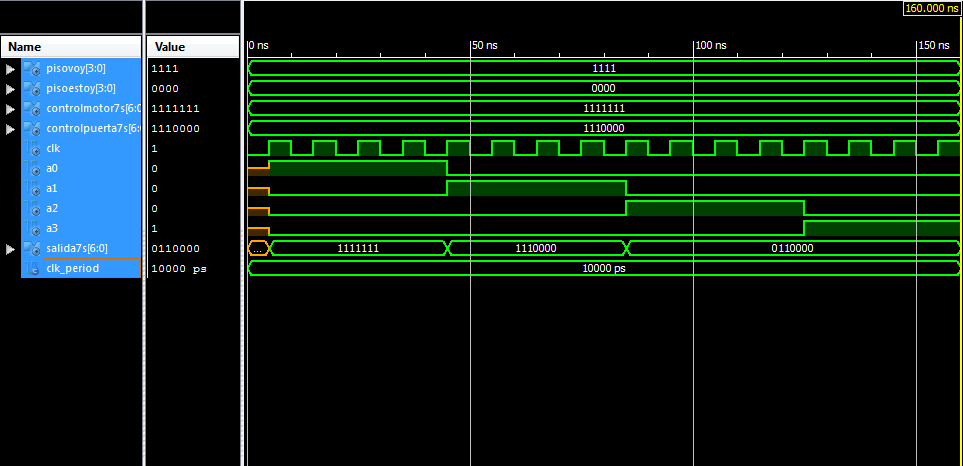
\includegraphics[width = 0.8\textwidth ]{SimulacionEntidadVisualizacion}
		    \caption{Simulación del testbench de la entidad Visualizacion}
		    \label{fig:SimulacionEntidadVisualizacion}
	\end{figure}

\subsection {Código Bloque \textit{DecodificadoLED} :} \label{code:DecodificadorLED}
	En este bloque vamos a mostrar en los ocho led de la FPGA el estado de los dos pisos almacenados, informando asi al usuario. Estos LEDs son activos a nivel lógico alto. Tenemos un toral de 8, hemos repartido los cuatro primeros para el primer piso almacenado y los cuatro siguientes para el segundo; empezanado a contar desde la derecha.
	\inputminted[frame=lines,fontsize=\footnotesize,linenos]{vhdl}{CodeFiles/DecodificadorLED.vhd}

	Como se puede ver en la Figura (\ref{fig:DecodificadorLEDOK}) el esquema obtenido una vez programado y sintetizado se corresponde con el que se pretendía.
    \begin{figure}[H]
		    \centering
		    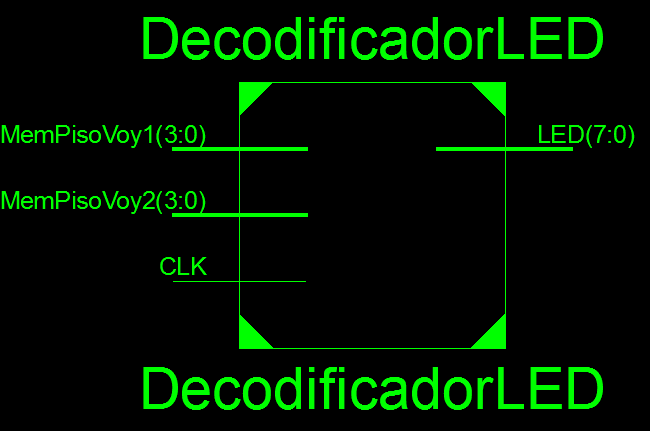
\includegraphics[width = 0.6\textwidth ]{DecodificadorLEDOK}
		    \caption{Esquema exterior del Bloque Decodificador LED}
		    \label{fig:DecodificadorLEDOK}
	\end{figure}
    Además podemos ver en la Figura (\ref{fig:DecodificadorLEDImplementacion}) como se compone internamente el bloque, como se codifica en hardware esta utilidad:
    \begin{figure}[H]
		    \centering
		    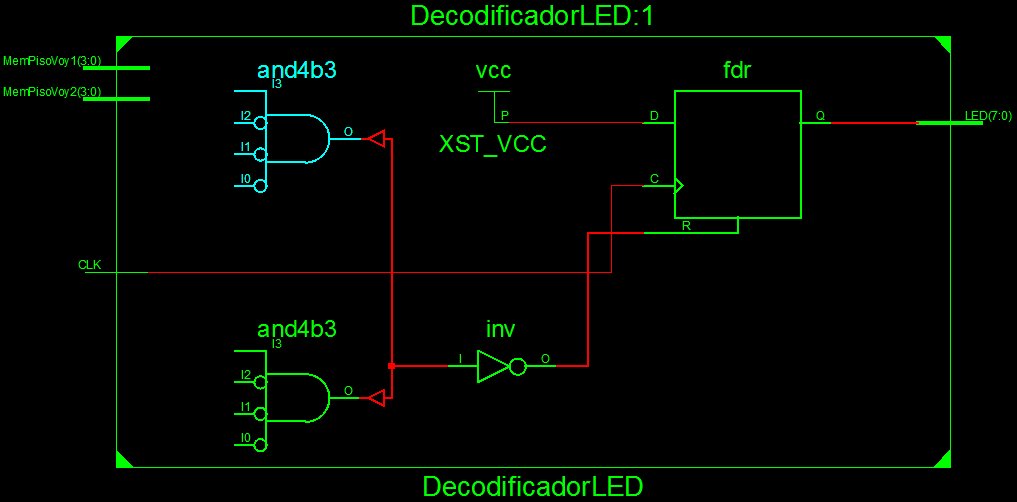
\includegraphics[width = 0.9\textwidth ]{DecodificadorLEDImplementacion}
		    \caption{Esquema interno del Bloque Decodificador LED}
		    \label{fig:DecodificadorLEDImplementacion}
	\end{figure}
	
\subsection {Código Bloque \textit{DecodificadoLED (testbench)} :} \label{code:DecodificadorLED_tb}
	\inputminted[frame=lines,fontsize=\footnotesize,linenos]{vhdl}{CodeFiles/DecodificadorLED_tb.vhd}

    Utilizando este testbench se obtiene el comportamiento que se puede ver en la Figura (\ref{fig:SimulacionDecodificadorLED}):

    \begin{figure}[H]
		    \centering
		    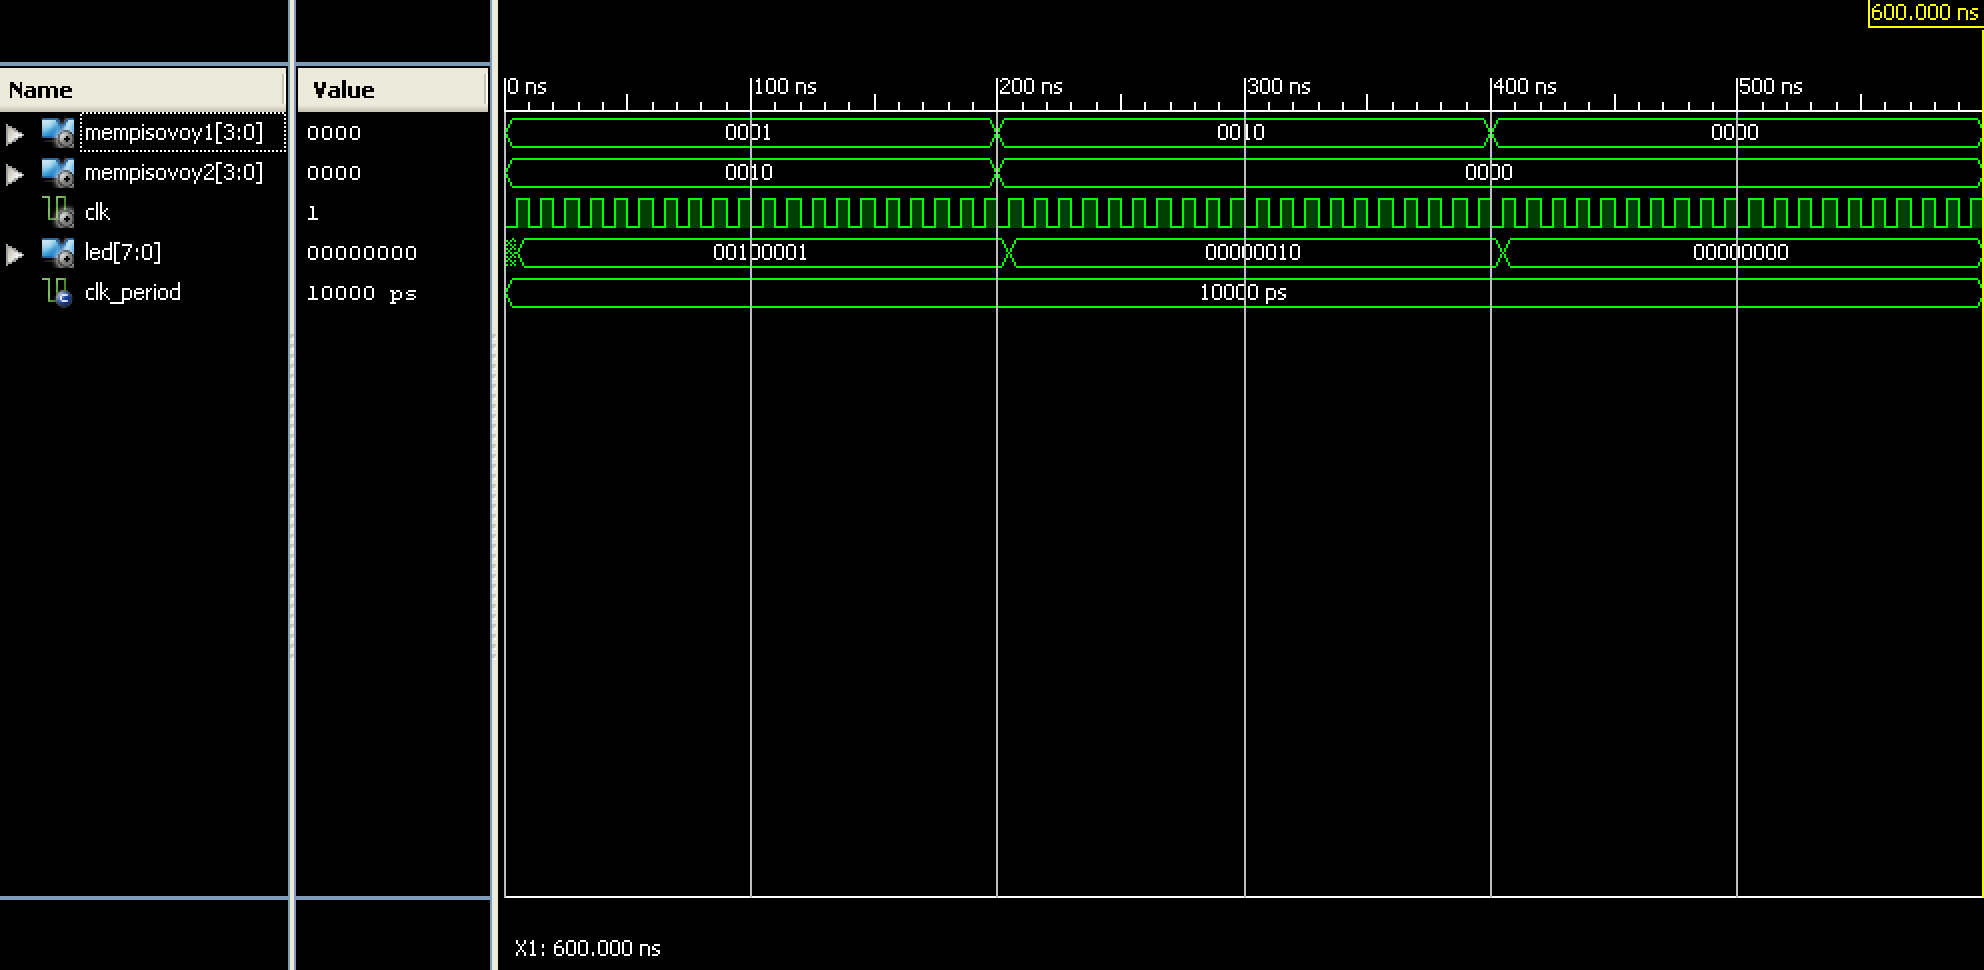
\includegraphics[width = 0.8\textwidth ]{SimulacionDecodificadorLED}
		    \caption{Simulación del testbench del DecodificadorLED}
		    \label{fig:SimulacionDecodificadorLED}
	\end{figure}
\subsection{Código Código Entidad \textit{Acensor}:} \label{code:Acensor}
Esta entidad,engobamos todas las anteriores para obtner asi funcinonamiento compoento de nuestro ascensor. \\ 
	\inputminted[frame=lines,fontsize=\footnotesize,linenos]{vhdl}{CodeFiles/EntidadAscensor.vhd}

	Como se puede ver en la Figura (\ref{fig:EntidadAscensorOK}) el esquema obtenido una vez programado y sintetizado se corresponde con el que se pretendía.
    \begin{figure}[H]
		    \centering
		    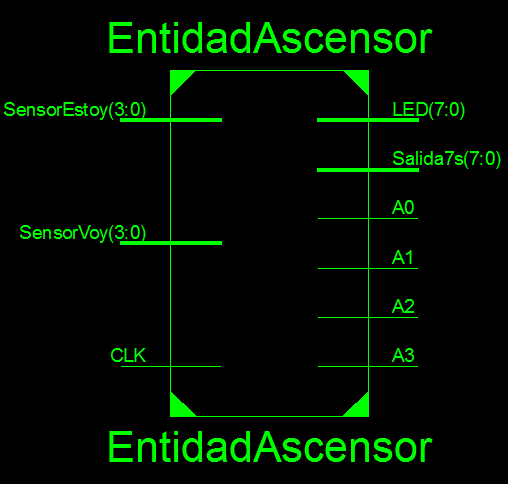
\includegraphics[width = 0.6\textwidth ]{EntidadAscensorOK}
		    \caption{Esquema exterior de la EntidadAscensor}
		    \label{fig:EntidadAscensorOK}
	\end{figure}
    Además podemos ver en la Figura (\ref{fig:EntidadAscensorImplementacion}) como se compone internamente el bloque, como se codifica en hardware esta utilidad:
    \begin{figure}[H]
		    \centering
		    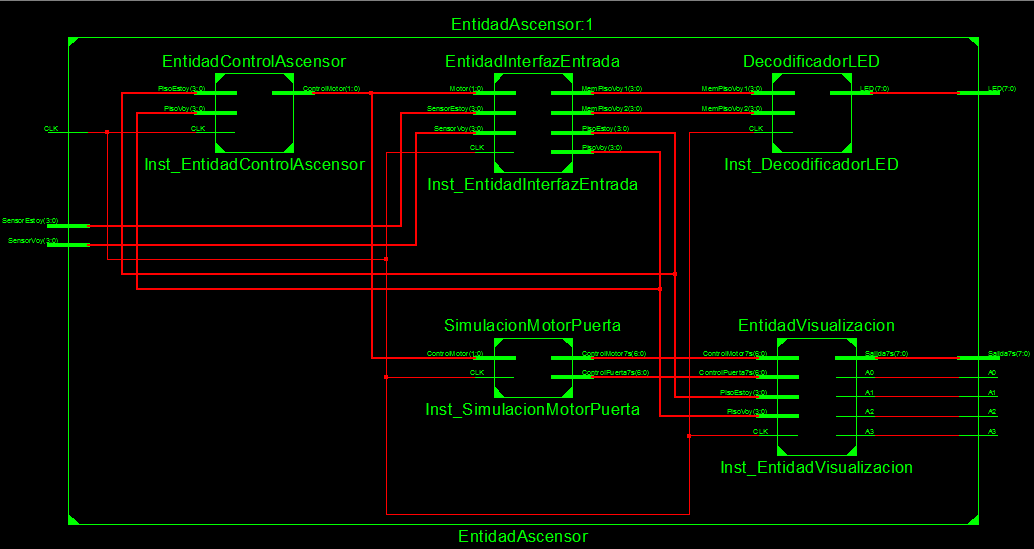
\includegraphics[width = 0.9\textwidth ]{EntidadAscensorImplementacion}
		    \caption{Esquema interno de la EntidadAscensor}
		    \label{fig:EntidadAscensorImplementacion}
	\end{figure}

\subsection{Código Código Entidad \textit{Acensor (testbench)}:} \label{code:Acensor_tb}
\inputminted[frame=lines,fontsize=\footnotesize,linenos]{vhdl}{CodeFiles/EntidadAscensor_tb.vhd}

    Utilizando este testbench se obtiene el comportamiento que se puede ver en la Figura (\ref{fig:SimulacionEntidadAscensor}):

    \begin{figure}[H]
		    \centering
		    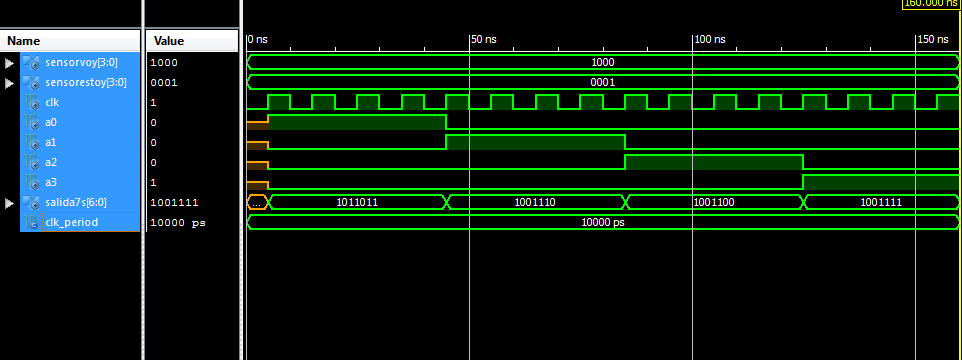
\includegraphics[width = 0.8\textwidth ]{SimulacionEntidadAscensor(Subiendo)}
		    \caption{Simulación del testbench de la entidad SimulacionEntidadAscensor(Subiendo)}
		    \label{fig:SimulacionEntidadAscensor}
	\end{figure}
